\zexternaldocument{inleiding}
\zexternaldocument{analyse}
\zexternaldocument{imp}

\chapter{Evaluatie}
\label{sec:evaluatie}
Om de impact van de verschillende heuristieken te meten volgt nu een overzicht van de testresultaten.
Voor het merendeel van de testen is een simulator gebruikt.
Sectie \ref{sec:simulator} legt uit waarom een simulator gebruikt wordt in plaats van IMP zelf, en hoe deze werkt.

De daarop volgende secties bespreken de resultaten van elke heuristiek. 
De algemene verwachting is dat het gebruik van heuristieken het aantal deployment runs reduceert en zo ook de totale uitroltijd.
Deze optimalisatie kost wel extra verwerkingstijd (de uitvoering van de verschillende heuristieken) maar deze is normaal gezien te verwaarlozen ten opzichte van het volledige uitrolproces.\todo{meten} 

\section{Simulator}
\label{sec:simulator}
Als deel van deze thesis werd een simulator voor IMP ontwikkeld.
Deze heeft een belangrijk aandeel in het evalueren van de ontwikkelde heuristieken.
Ze laat namelijk toe op een snelle en eenvoudige manier een uitgebreid model uit te rollen en geeft volledige controle over welke informatie tijdens dat proces beschikbaar wordt gesteld aan de gebruiker.
De snelheid en eenvoud van de simulator in vergelijking met op fysieke hosts uitrollen is te danken aan twee redenen:

ten eerste is de uitroltijd evenredig met het aantal resources in het model.
Elke resource moet verwerkt worden, en vooral pakketten duren lang om uit te rollen. 
Deze moeten niet alleen gedownload worden maar ook ge\"installeerd, beide taken kunnen aardig wat tijd innemen.
Bij de simulator komt het uitrollen van een pakket overeen met het wegschrijven van een reeks waarden in een database, wat significant sneller is.
Hierbij moet wel een kanttekening gemaakt worden: bij fysiek uitrollen wordt het uitrollen van het model verdeeld over de verschillende hosts, elk zijn eigen deel van het model.
De simulator moet alle resources van alle hosts alleen verwerken. 
Zelfs dan nog is de snelheidswinst bij de simulator significant.

Ten tweede laat een simulator toe modellen met honderden machines uit te rollen op \'e\'en enkele pc.
Naarmate de modellen groter worden wordt het steeds moeilijker het model op fysieke hosts te testen.
En het zijn juist de grotere modellen, met meer hosts, die interessant zijn voor de evaluatie van de heuristieken.

De simulator bootst een systeem na dat Fedora 18 draait en gebruik maakt van de yum pakket manager.

\subsection{Uitwerking}
\label{simulator:uitwerking}
De simulator is een Pythonscript dat als invoer een JSON-bestand met daarin het gecompileerde model.
IMP zelf stelt dit bestand op als de optie ``-j [naam JSON]'' wordt meegegeven.
Tijdens het uitvoeren van dit script wordt een sqlite-database opgesteld.
De tabellen van deze database zijn te zien in de tabellen \ref{table:deploymentdatabase}.

\begin{table}[h]
\centering
\begin{tabular}[t]{ |l|l| }
  \hline
  \multicolumn{2}{|c|}{Agent} \\
  \hline
  name & Text \\
  \hline
\end{tabular}
\quad
\begin{tabular}[t]{ |l|l| }
  \hline
  \multicolumn{2}{|c|}{Attribute} \\
  \hline
  name & Text \\
  value & Text \\
  ResourceId & Text \\
  \hline
\end{tabular}
\quad
\begin{tabular}[t]{ |l|l| }
  \hline
  \multicolumn{2}{|c|}{Resource} \\
  \hline
  Id & Text \\
  \hline
\end{tabular}
\caption{De verschillende tabellen die aanwezig zijn in de deploymentdatabase.}
\label{table:deploymentdatabase}
\end{table}

In de Attribute tabel staan de attributen opgeslagen als volgt:
\begin{verbatim}
name     value       ResourceId                                                                                          
-------- ---------- ---------------------------------------------------
group    root        std::File[server,path=/tmp/test],v=1389435342             
owner    root        std::File[server,path=/tmp/test],v=1389435342             
path     /tmp/test   std::Directory[server,path=/tmp/test],v=1389435342                        
\end{verbatim}

Om de simulatie zo waarheidsgetrouw mogelijk te maken houdt de simulator rekening met volgende aspecten van het fysieke uitrolproces:

\begin{itemize}
  \item Bestanden en mappen kunnen niet aangemaakt worden voordat de bovenliggende map bestaat.
  \item Services kunnen niet gestart worden voordat het bijhorende pakket en bestanden aanwezig zijn.
  \item Resources worden pas aangemaakt als hun afhankelijkheden voldaan zijn.
\end{itemize}

Nakijken of alle bijhorende pakketten en bestanden van een service aanwezig zijn wordt gebruikt gemaakt van de repositorydata van de yum pakketmanager.
De repositorydata bevat twee handige databases: de primary en de filelists.
De relevante attributen de gebruikte tabellen zijn te vinden in tabel \ref{table:repodata}.

\begin{table}[h]
\centering
\begin{tabular}[t]{ |l|l| }
  \hline
  \multicolumn{2}{|c|}{packages} \\
  \hline
  pkgKey & Integer \\
  name & Text \\
  \hline
\end{tabular}
\quad
\begin{tabular}[t]{ |l|l| }
  \hline
  \multicolumn{2}{|c|}{filelist} \\
  \hline
  pkgKey & Integer \\
  name & Text \\
  dirname & Text \\
  filenames & Text \\
  \hline
\end{tabular}
\caption{De relevante attributen van de repositorydatabases die gebruikt worden door de simulator}
\label{table:repodata}
\end{table}

De uiteindelijke database die gebruikt wordt door te simulator bestaat uit de samenvoeging van de attributen uit de twee databases.
Aangezien sommige pakketten een eigen yum repository hebben is voor die gevallen manueel de repositorydata toegevoegd.
Een voorbeeld van de data die zo bekomen wordt:

\begin{verbatim}
name          dirname                    filenames                     
------------  -------------------------  ------------------------------
oniguruma     /usr/lib                   libonig.so.2.0.0/libonig.so.2 
oniguruma     /usr/share/doc             oniguruma-5.9.2               
openCOLLADA   /usr/share/doc             openCOLLADA-0                 
\end{verbatim}

Bij het installeren van een pakket in de simulator wordt een lijst van alle bestanden en mappen die bij dat pakket horen opgesteld.
Elk element van deze lijst wordt als entry toegevoegd aan de Attribute tabel, met als value het pad naar dat bestand.
Als de simulator probeert een bepaalde service uit te rollen zoekt hij alle entries met de servicenaam en stelt een lijst met alle nodige bestanden en mappen op.
Daarna wordt in de Attribute tabel gecheckt of deze allemaal aanwezig zijn.

Naast de repositorydata wordt ook nog een lijst gebruikt met daarin de bestanden en mappen die standaard aanwezig zijn op een nieuwe Fedora 18 installatie.
Zonder deze lijst zou elke poging tot het uitrollen van een bestand of map falen, omdat voor geen enkel bestand de bovenliggende map bestaat.

In pseudecode ziet het uitrollen van elke type resource er uit als volgt:

\begin{lstlisting}[showstringspaces=false]
def deploy_file(file):
  #Check if parent folder exists already
  if parent(file) in std_filesystem or parent(file) in deployment_database:
    deployment_database.write(file)
  else:
    error('Parent folder doesn't exist!')

def deploy_service(srv):
  #Check if required files have been deployed
  requirements = repodata_database.execute('select * from pkgdata where name like srv.name')
  if all([req in deployment_database for req in requirements]):
    deployment_database.write(srv)
  else:
    error('Not all required resources were deployed!')

def deploy_package(pkg):
  pkg_files = repodata_database.execute('select * from pkgdata where name like pkg.name') 
  foreach file in pkg_files:
    deployment_database.write(file)
\end{lstlisting}

Bij het uitrollen van een pakket worden geen controles gedaan. 
De simulator gaat er van uit dat het correct uitrollen van een pakket de verantwoordelijkheid is van de pakketmanager, niet de CMS.

Om zo goed mogelijk een fysiek uitrolproces te simuleren gebruikt de simulator een gelijkaardig algoritme voor het uitrollen van het model.
Daarbij worden eerst alle resources weggeschreven die geen vereisten hebben.
Daarna wordt gekeken of de resources die net zijn uitgerold een vereiste waren van de overblijvende resources.
Als dit het geval is worden de geschreven resources verwijderd uit de lijst met vereisten.
Zo komen (hopelijk) nieuwe resources vrij die geen vereisten meer hebben en die kunnen in de volgende herhaling uitgerold worden.
Dit proces herhaalt zich tot er geen resources meer moeten uitgerold worden.

\todo{Verschil in uitroltijd simulator/IMP?}
\todo{Besluit sectie}

\section{Afhankelijkheden tussen bestanden en mappen}
\label{sec:bestanden_en_mappen_eval}
Aangezien een bestand niet kan gecre\"eerd worden zonder zijn bovenliggende map voegt deze heuristiek automatisch de afhankelijkheid tussen beide toe aan het model.

Aangezien mappen altijd kunnen gecre\"eerd worden zijn er maximaal twee deployment runs nodig als er geen heuristiek gebruikt wordt.\footnote{Twee runs als maar \'e\'en bovenliggende map moet aangemaakt worden. Per bijkomend niveau is mogelijks een extra run nodig.}
Bij gebruik van de heuristiek moet er exact \'e\'en uitgerold worden.
De verwachting is dat het uitrollen met gebruik van de heuristiek dan ook ongeveer half zo lang duurt.

Figuur \ref{fig:file_dir_times} toont de resultaten van deze test.
Elk datapunt is het gemiddelde van 30 runs, uitgevoerd op een virtuele machine met twee cores van 2Ghz en 2GB RAM ter beschikking.
Het model bestaat iedere keer uit een vast aantal bestanden en mappen, \'e\'en bestand per map.
\begin{figure}[h]
    \begin{center}
    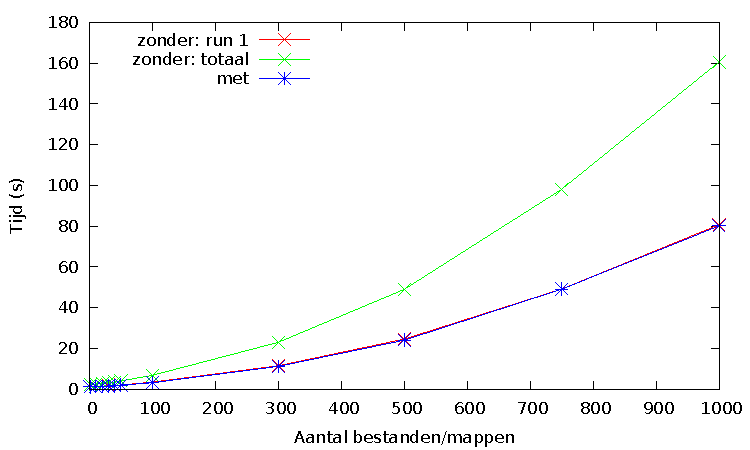
\includegraphics[width=0.8\textwidth]{images/file_dir_times.pdf}
    \caption{Testresultaten bij het uitrollen van een stijgend aantal bestanden en mappen, met en zonder gebruik van de heuristiek}
    \label{fig:file_dir_times}
    \end{center}
\end{figure}

De verwachtingen zijn volledig ingelost: zonder heuristiek zijn er twee deployment runs nodig, met heuristiek slechts \'e\'en.
Dit weerspiegelt zich in de gehalveerde uitroltijd.

\section{Afhankelijkheden tussen services, pakketten en configuratiebestanden}
\label{sec:stacks_eval}
De specificatie van een service in het configuratiemodel gaat vaak gepaard met de pakket en de configuratiebestanden die die service nodig heeft.
Deze combinatie van resources wordt een stack genoemd.
Aangezien de service niet correct werkt zonder de aanwezigheid van het pakket en de configuratiebestanden voegt deze heuristiek de gepaste vereisten toe aan het model.


Voor deze test moest IMP 30 keer de NTP service uitrollen op een testmachine.
NTP bestaat uit \'e\'en pakket, \'e\'en configuratiebestand en \'e\'en service. 
In het slechtste geval zijn er normaal gezien dus drie deployment runs nodig om de service correct werkende te krijgen.
Als de correcte afhankelijkheden worden opgesteld is er slechts \'e\'en run nodig.
De testresultaten zijn te vinden in tabel \ref{table:service_package_dep}.

\begin{table}
  \begin{center}
  \begin{tabular}{ r | c | c }
            & tijd(s)   & gemiddeld aantal runs nodig \\ \hline
    zonder  & 3.21      & 2.0 \\ \hline
    met     & 2.21      & 1 \\
  \end{tabular}
  \caption{Meetresultaten}
  \label{table:service_package_dep}
  \end{center}
\end{table}
%specifieke resultaten:
%zonder
%Avg time: 3.212880388398965
%Deployments avg: 2.0
%met: Avg time: 2.2067235755423704
%deps toegevoegd: 3

De resultaten van de test zijn zoals verwacht: dankzij de heuristiek is maar \'e\'en deployment run nodig.

\section{Relaties en afhankelijkheden tussen hoog-niveau concepten}
De heuristieken uit sectie \ref{sec:relaties} en \ref{sec:vereisten_uit_afhankelijkheden} werken best samen.
De eerste vormt relaties met een bepaalde multipliciteit om naar afhankelijke relaties.
De tweede zet afhankelijke relaties tussen entiteiten die services bevatten om naar vereisten tussen die services.
Zo wordt vermeden dat een extra deployment run nodig is de services correct op te starten.

Deze heuristieken werden niet apart getest, enkel in de use cases.
In individuele testen zouden de resultaten gelijkaardig zijn aan die van de bestanden en mappen heuristiek.

\section{Use cases}

\subsection{Document processing}
Deze eerste use case studie betreft een uitgebreide en complexe infrastructuur gebruikt voor de geautomatiseerde verwerking van documenten.
De infrastructuur ondersteunt \todo{cite} de creatie, het opstellen van de layout, de processing en het opslaan van bedrijfsdocumenten (bvb facturen, orders, aandelen,\ldots).
Ze wordt meestal uitgerold als een cloudservice.
Figuur \ref{fig:doc_processing} toont de verschillende onderdelen van deze opstelling:
de gebruiker kan via verschillende inputkanalen data doorspelen aan de productieservice.
Die verwerkt de gegevens in verschillende stappen.
De worker nodes zijn verantwoordelijk voor de verwerking van die acties.
De resultaten worden geplaatst in een database en kunnen via verschillende outputkanalen opgevraagd worden.

\begin{figure}[h]
    \begin{center}
    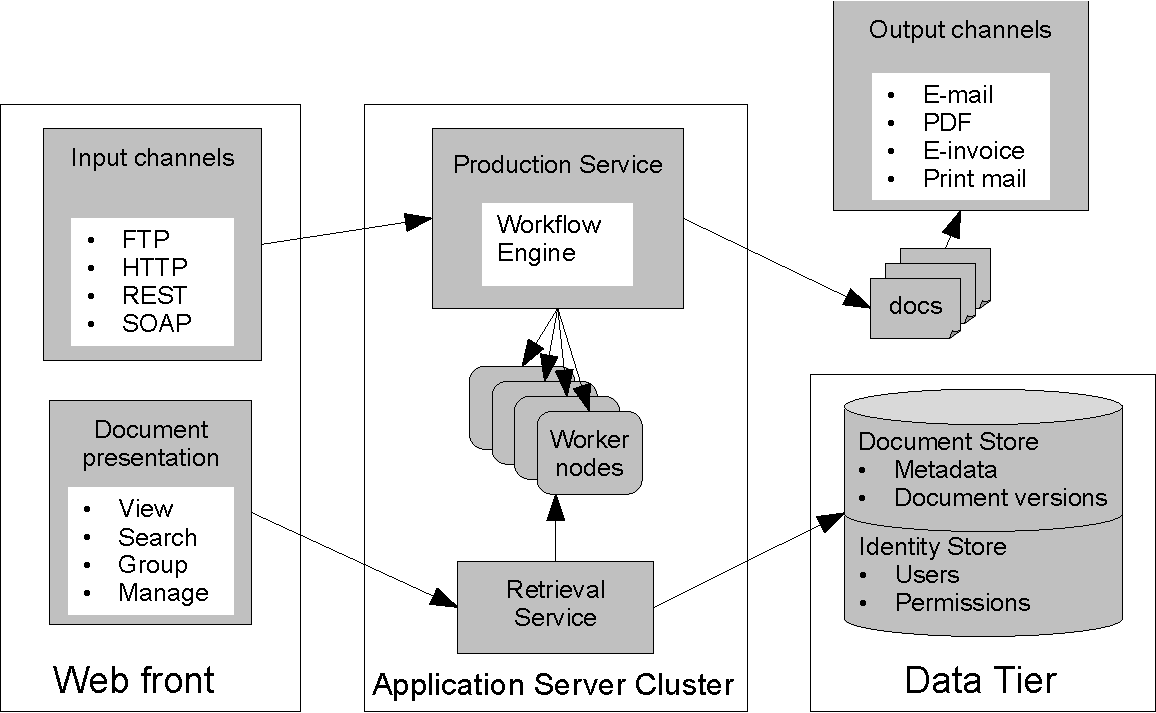
\includegraphics[width=0.8\textwidth]{images/doc_processing.pdf}
    \caption{Overzicht van de document processing infrastructuur}
    \label{fig:doc_processing}
    \end{center}
\end{figure}

Het volledige model in IMP van deze use case bestaat uit 35 bibliotheken \todo{bibliotheken vermelden, mogelijks een hoofdstuk introductie tot IMP?} waaronder Apache, HBase, Cassandra, \ldots
In totaal zijn er reeds 82 relaties gespecifi\"eerd, maar het model is nog niet volledig.

\todo{Dit is eigenlijk geen uitleg van de toepassing van de heuristieken op de use case, meer een uitleg/test van de heuristieken}
In afbeelding \ref{fig:reqs_doc} is te zien hoeveel vereisten elke heuristiek toevoegen.
De heuristiek die de bovenliggende map toevoegt aan de vereisten van een map of bestand wordt altijd uitgevoerd.
Deze heuristiek beschouwen we namelijk als fundamenteel: de vereisten die ze toevoegd zijn sowieso juist, terwijl sommige vereisten die door andere heuristieken worden toegevoegd mogelijks overbodig zijn. 

De verwachting is dat sommige heuristieken zullen overlappen, bijvoorbeeld ``stack'' en ``name''. 
Resources binnen dezelfde stack hebben namelijk vaak een gelijkaardige naam. 

\begin{figure}[h]
    \begin{center}
    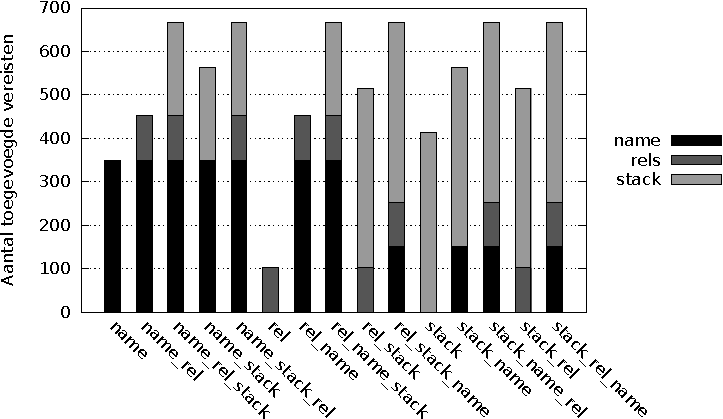
\includegraphics[width=0.8\textwidth]{images/reqs_doc.pdf}
    \caption{Aantal toegevoegde vereisten voor elke combinatie van heuristieken in de document processing use case}
    \label{fig:reqs_doc}
    \end{center}
\end{figure}

Als een bepaalde heuristiek eerst toegepast wordt kan hij al zijn vereisten toevoegen.
Daaropvolgende heuristieken zullen enkel het deel van hun vereisten toevoegen die nog niet deel uitmaken van het model.
Ongeacht de volgorde zal een combinatie heuristieken altijd dezelfde set vereisten toevoegen.

In afbeelding \ref{fig:time_runs_doc} is te zien welke impact de toegevoegde vereisten hebben op het uitrolproces.

\begin{figure}[h]
    \begin{center}
    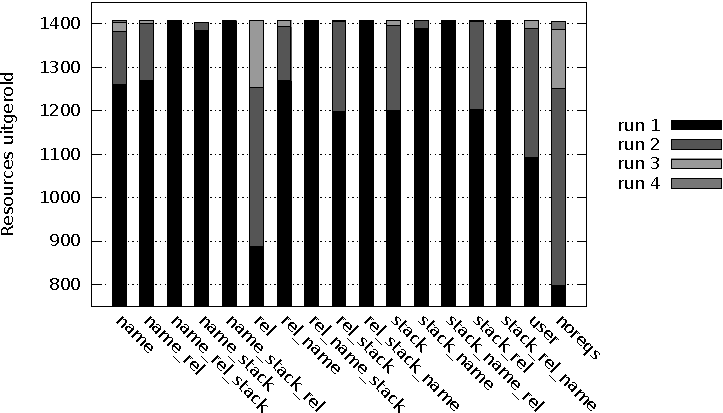
\includegraphics[width=0.8\textwidth]{images/time_runs_doc.pdf}
    \caption{Gemiddelde aantal uitgerolde resources per deployment run voor elke combinate van heuristieken in de document processing use case}
    \label{fig:time_runs_doc}
    \end{center}
\end{figure}

De resultaten bevestigen onze aanname dat het toevoegen van vereisten kan leiden tot een daling in het aantal deployment runs.
Elke combinatie van de drie heuristieken leidt zelfs tot een ``one-shot'' uitrolproces waarin in \'e\'en keer het volledige model correct uitgerold wordt.

Het volledige model bevat 82 relaties. 
\subsection{MongoDB}
MongoDB is een van de meer bekende NoSQL databases.
Een volledige configuratie bestaat uit verschillende services die elkaar ondersteunen.
Figuur \ref{fig:mongodb_architecture} geeft een schematische voorstelling van een dergelijke set-up. \todo{cite}

\begin{figure}[h]
    \begin{center}
    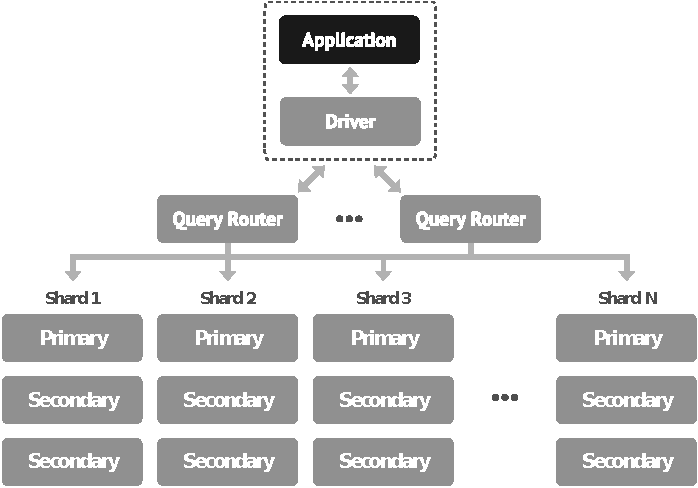
\includegraphics[width=0.8\textwidth]{images/mongodb_architecture.pdf}
    \caption{Architectuur van de MongoDB database}
    \label{fig:mongodb_architecture}
    \end{center}
\end{figure}

In het model dat Thomas Uyttendaele opgesteld heeft \todo{cite} krijgen de onderdelen de volgende namen:

\begin{table}[h!]
  \begin{center}
  \begin{tabular}{c | c}
  Query Router  & AccessServer \\ \hline
  Primary       & ReplicaSetController \\ \hline
  Secondary     & Node \\ 
  \end{tabular}
  \end{center}
\end{table}

De onderdelen zullen pas correct kunnen samenwerken als ze in de juiste volgorde worden opgestart.
Figuur \ref{fig:mongo_imp} toont de implementatie van MongoDB in IMP, samen met de volgorde waarin de services gestart moeten worden.

\begin{figure}[h]
    \begin{center}
    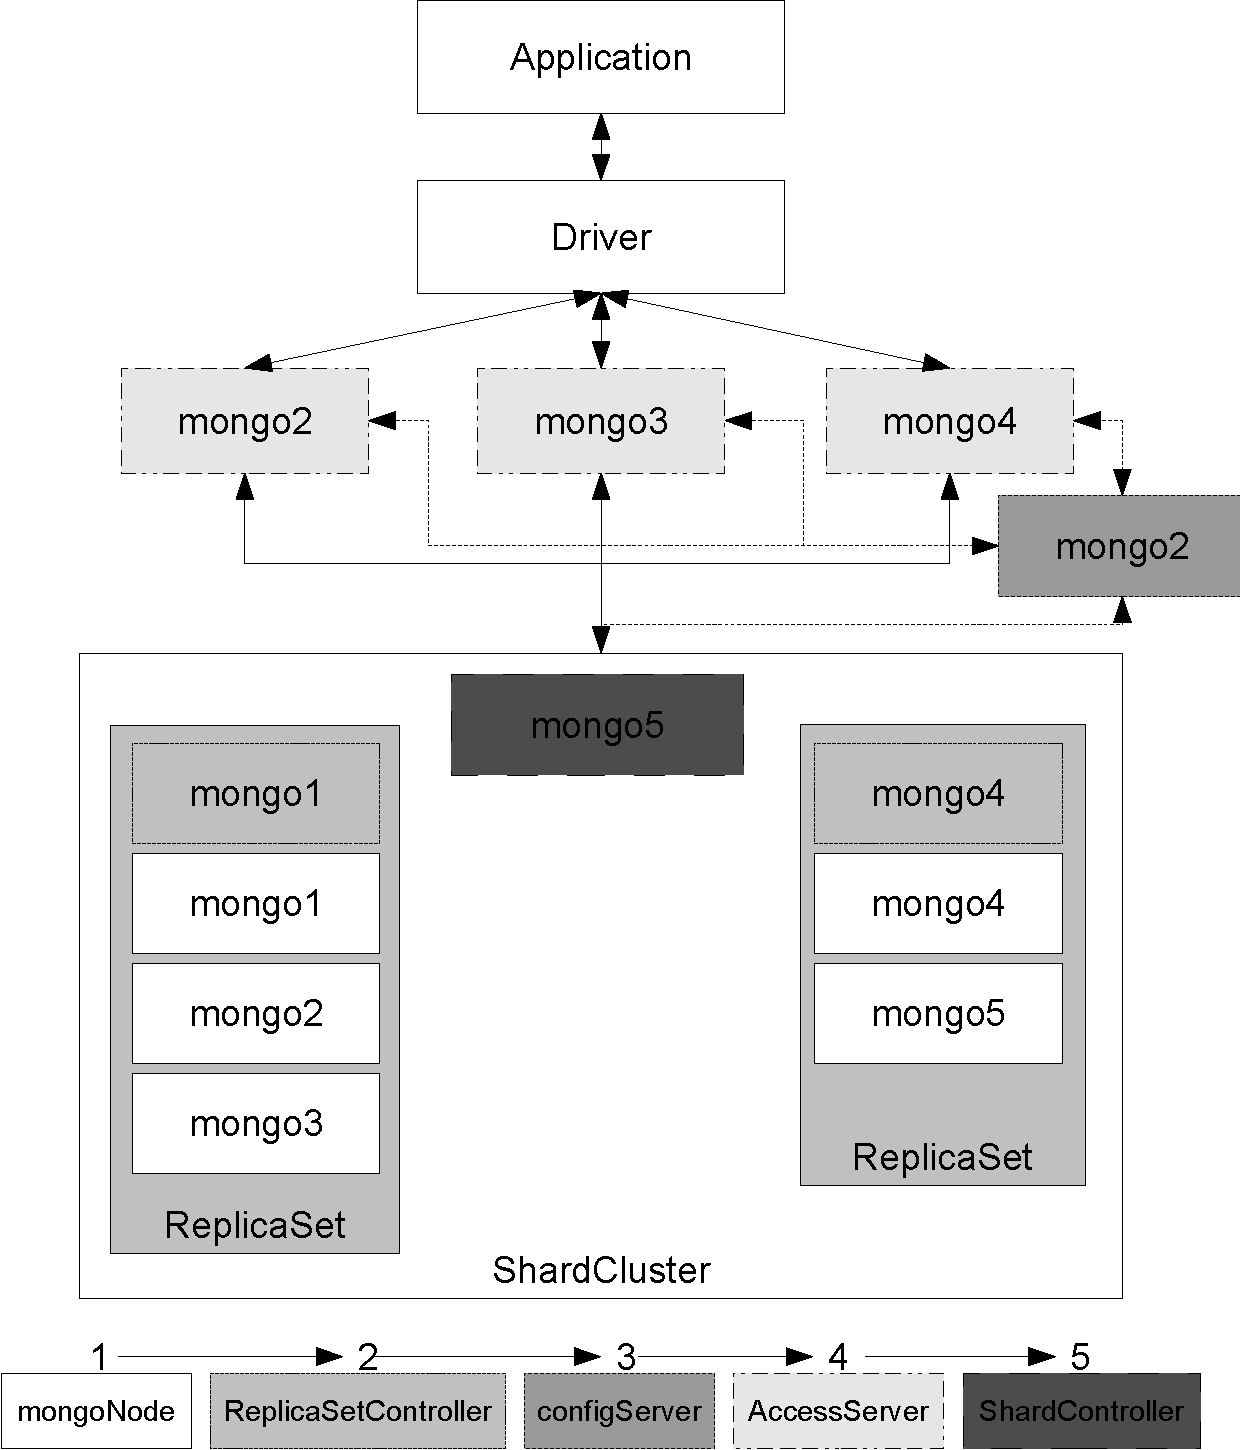
\includegraphics[width=0.8\textwidth]{images/mongo_imp.pdf}
    \caption{Implementatie van MongoDB in IMP, met de correcte opstartvolgorde aangeduid}
    \label{fig:mongo_imp}
    \end{center}
\end{figure}

Het is dus weerom \todo{Vroeger vermelden dat het van groot belang is dat het model compleet is} van groot belang dat alle afhankelijkheden in het model
vermeld worden.

Voor de volgende resultaten werd een instantie van MongoDB uitgerold met vijf nodes, verdeeld in twee replicasets van twee en drie nodes elk.
Drie nodes nemen ook de rol van Query Router op zich.
Figuur \ref{fig:reqs_mongo} toont de vereisten die elke combinatie van heuristieken toevoegt.

\begin{figure}[h]
    \begin{center}
    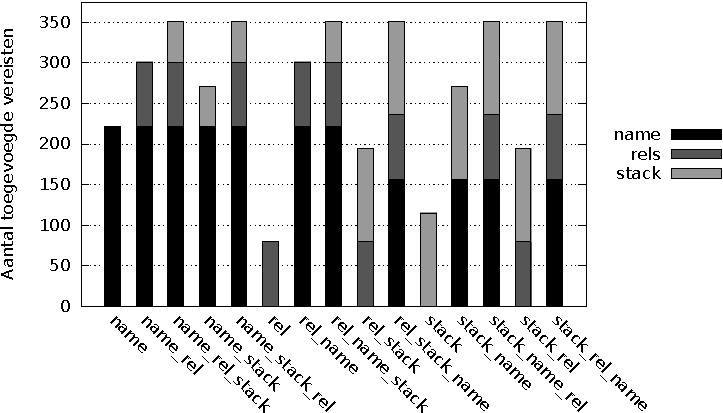
\includegraphics[width=0.8\textwidth]{images/reqs_mongo.pdf}
    \caption{Aantal toegevoegde vereisten voor elke combinatie van heuristieken bij MongoDB}
    \label{fig:reqs_mongo}
    \end{center}
\end{figure}

Figuur \ref{fig:time_runs_mongo} toont hoeveel deployment runs nodig zijn om een volledig werkende MongoDB database te bekomen, en hoeveel resources er
per run gedeployed worden.

\begin{figure}[h]
    \begin{center}
    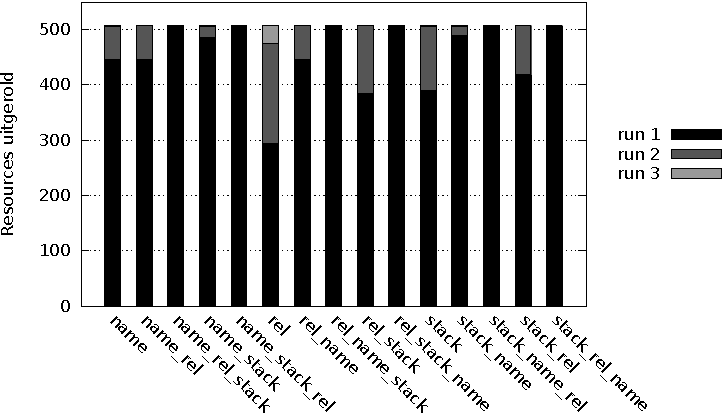
\includegraphics[width=0.8\textwidth]{images/time_runs_mongo.pdf}
    \caption{Gemiddelde aantal uitgerolde resources per deployment run voor elke combinate van heuristieken bij MongoDB}
    \label{fig:time_runs_mongo}
    \end{center}
\end{figure}

De library voor MongoDB bestaat uit 185 regels code\footnote{Blanco lijnen en commentaar niet meegerekend}, waarvan er 24 relaties beschrijven.
Alle libraries samen bevatten 50 relaties. 
